\documentclass[12pt, twoside]{article}
\input{../preamble}

\fancyhead[LO]{La Scuola d'Italia / Dr.\ Huson / IB Math 12 \\* 9 September 2026}
\fancyhead[RO]{\fbox{\begin{minipage}{6cm}\footnotesize First \& Last name:\\[0.5cm]\end{minipage}}}
\fancyfoot[C]{\thepage}

\begin{document}
\subsubsection*{2.1 Classwork: Exponential Functions Review}

\begin{enumerate}[itemsep=0.15cm]

%--- Problem 1: Exponential graph --- asymptote, intercepts, sketch [7 marks] ---
%--- Source: Original (authored September 2026) ---
\item[1.] [Maximum mark: 7]

Consider the function $f(x) = 3 \cdot 2^{\,x} - 5$.

\begin{enumerate}[itemsep=0.1cm]
  \item Write down the equation of the horizontal asymptote of the
  graph of $f$. \hfill [1]
  \item Find the $y$-intercept of the graph of $f$. \hfill [1]
  \item Find $f(4)$. \hfill [1]
  \item Find the $x$-intercept of the graph of $f$, correct to three
  significant figures. \hfill [2]
  \item On the axes below, sketch the graph of $f$ for
  $-3 \le x \le 2$, showing the horizontal asymptote and both
  intercepts. \hfill [2]
\end{enumerate}

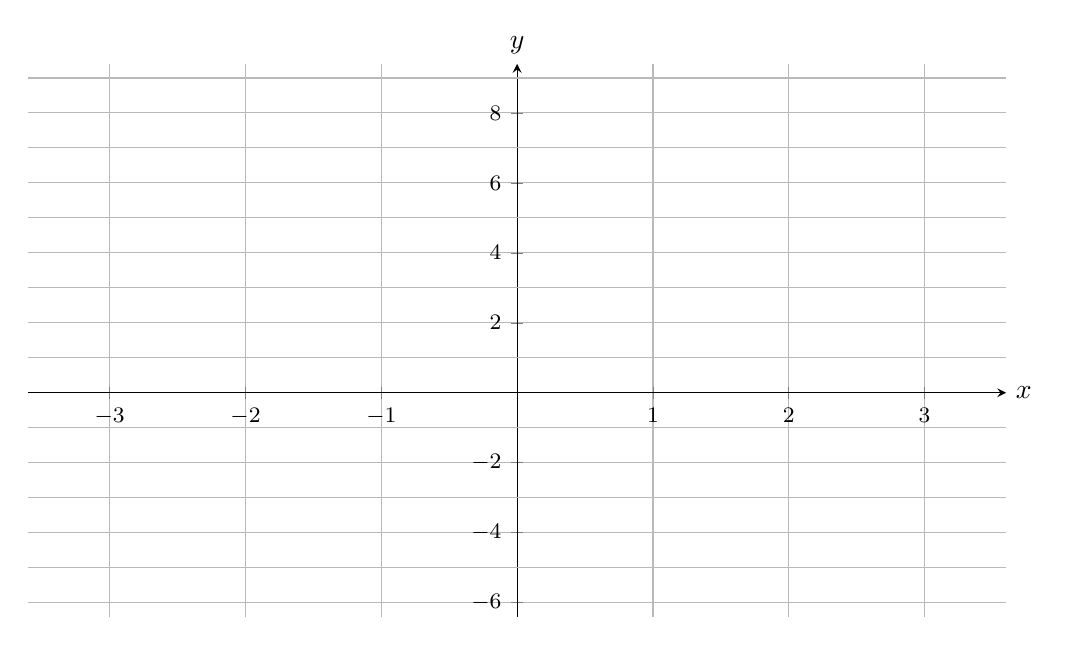
\begin{tikzpicture}
\begin{axis}[
  axis lines=middle,
  xlabel={$x$}, ylabel={$y$},
  xlabel style={anchor=west}, ylabel style={anchor=south},
  xmin=-3.6, xmax=3.6, ymin=-6.4, ymax=9.4,
  xtick={-3,-2,-1,1,2,3},
  ytick={-6,-4,-2,2,4,6,8},
  extra y ticks={-5,-3,-1,1,3,5,7,9},
  extra y tick labels={},
  extra y tick style={grid=major, tick style={draw=none}},
  tick label style={font=\footnotesize},
  grid=major,
  major grid style={gray!55},
  width=14cm, height=8.6cm,
]
  % Solution curve (drawn in the markscheme only):
  % \addplot[thick, smooth, samples=200, domain=-3.6:2.17] {3*2^x - 5};
  % \addplot[dashed, domain=-3.6:3.6] {-5};
\end{axis}
\end{tikzpicture}

\begin{center}
\begin{tikzpicture}
  \draw (-0.6,0) rectangle (11,6.2);
  \foreach \y in {1,2,...,6} \draw[dotted] (0,\y)--(10.5,\y);
\end{tikzpicture}
\end{center}

\newpage

%--- Problem 2: Solving exponential equations with logarithms [6 marks] ---
%--- Source: Original (authored September 2026) ---
\item[2.] [Maximum mark: 6]

Solve each equation for the unknown, showing your working with
logarithms. Give each answer correct to three significant figures.

\begin{enumerate}[itemsep=0.1cm]
  \item $5^{\,x} = 300$ \hfill [2]
  \item $20\, e^{\,0.15 t} = 90$ \hfill [2]
  \item $2^{\,x+1} = 3^{\,x}$ \hfill [2]
\end{enumerate}

\begin{tikzpicture}
  \draw (-0.6,0) rectangle (11,17);
  \foreach \y in {1,2,...,16} \draw[dotted] (0,\y)--(10.5,\y);
\end{tikzpicture}

\newpage

%--- Problem 3: Continuous growth model N = N_0 e^{kt} [7 marks] ---
%--- Source: Original (authored September 2026) ---
\item[3.] [Maximum mark: 7]

The number of electric cars registered in a city is modelled by
$$N(t) \;=\; N_{0}\, e^{\,k t}, \qquad k > 0,$$
where $t$ is the number of years after the start of 2020. At the start
of 2022 there were $4500$ electric cars registered, and at the start of
2026 there were $7200$.

\begin{enumerate}[itemsep=0.1cm]
  \item Find the value of $k$, correct to three significant figures.
  \hfill [2]
  \item Find the value of $N_{0}$, correct to the nearest whole number.
  \hfill [1]
  \item The model predicts that the number of registered electric cars
  grows by a fixed percentage each year. Find this annual percentage
  growth rate, correct to three significant figures. \hfill [1]
  \item Use the model to predict the number of registered electric cars
  at the start of $2030$, correct to the nearest whole number.
  \hfill [1]
  \item Find the value of $t$ at which the number of registered
  electric cars first reaches $15\,000$. Give your answer correct to
  three significant figures. \hfill [2]
\end{enumerate}

\begin{tikzpicture}
  \draw (-0.6,0) rectangle (11,11.5);
  \foreach \y in {1,2,...,11} \draw[dotted] (0,\y)--(10.5,\y);
\end{tikzpicture}

\newpage

%--- Problem 4: Compound interest, doubling time, overtaking [6 marks] ---
%--- Source: Original (authored September 2026) ---
\item[4.] [Maximum mark: 6]

Ana invests \$2000 in an account paying interest of $4.5\,\%$ per
annum, compounded annually. The value of her investment after $n$
years is given by the formula
$$\mathit{FV} \;=\; \mathit{PV} \left(1 + \dfrac{r}{100}\right)^{\!n},$$
where $\mathit{PV}$ is the amount invested and $r$ is the annual interest rate.
No further deposits or withdrawals are made.

\begin{enumerate}[itemsep=0.1cm]
  \item Find the value of Ana's investment after $8$ years, correct to
  the nearest cent. \hfill [1]
  \item Find the smallest whole number of years after which Ana's
  investment is worth at least twice the amount she invested.
  \hfill [2]
\end{enumerate}

On the same day, Ben invests \$3000 in an account paying interest of
$2\,\%$ per annum, compounded annually.

\begin{enumerate}[itemsep=0.1cm]
  \item[(c)] Find the smallest whole number of years after which Ana's
  investment is worth more than Ben's. \hfill [3]
\end{enumerate}

\begin{tikzpicture}
  \draw (-0.6,0) rectangle (11,12);
  \foreach \y in {1,2,...,11} \draw[dotted] (0,\y)--(10.5,\y);
\end{tikzpicture}

\end{enumerate}
\end{document}
